\documentclass[12pt,a4paper]{article}
\usepackage[utf8]{inputenc}
\usepackage[T1]{fontenc}
\usepackage{graphicx}
\usepackage{listings}
\usepackage{xcolor}
\usepackage{amsmath}
\usepackage{hyperref}
\usepackage{geometry}
\usepackage{tikz}
\usetikzlibrary{shapes.geometric, arrows, positioning, shadows, calc}
\geometry{margin=1in}

% --- TikZ Styles ---
\tikzstyle{block} = [rectangle, draw, fill=blue!20, text width=5em, text centered, rounded corners, minimum height=4em, drop shadow]
\tikzstyle{attacker} = [rectangle, draw, fill=red!20, text width=5em, text centered, rounded corners, minimum height=4em, drop shadow]
\tikzstyle{line} = [draw, -latex', thick]
\tikzstyle{state} = [circle, draw, fill=green!20, text width=4em, text centered, minimum height=4em, node distance=5.5cm]

% --- Listings Setup for Code ---
\definecolor{codegreen}{rgb}{0,0.6,0}
\definecolor{codegray}{rgb}{0.5,0.5,0.5}
\definecolor{codepurple}{rgb}{0.58,0,0.82}
\definecolor{backcolour}{rgb}{0.95,0.95,0.92}

\lstdefinestyle{mystyle}{
    backgroundcolor=\color{backcolour},   
    commentstyle=\color{codegreen},
    keywordstyle=\color{magenta},
    numberstyle=\tiny\color{codegray},
    stringstyle=\color{codepurple},
    basicstyle=\ttfamily\footnotesize,
    breakatwhitespace=false,         
    breaklines=true,                 
    captionpos=b,                    
    keepspaces=true,                 
    numbers=left,                    
    numbersep=5pt,                  
    showspaces=false,                
    showstringspaces=false,
    showtabs=false,                  
    tabsize=2
}
\lstset{style=mystyle}

\begin{document}

% ---------------------------------------------------------
% 1. Cover Page
% ---------------------------------------------------------
\begin{titlepage}
    \centering
    \vspace*{1cm}
    
    {\Huge \textbf{Secure UART: End-to-End Encrypted Communication}} \\
    \vspace{1.5cm}
    
    {\Large \textbf{Digital System Interfacing}} \\
    {\large Course Code: DSI} \\
    \vspace{1.5cm}
    
    \textbf{Student Names \& IDs:} \\[0.5cm]
    Youssef Basem (240919) \\
    Moaaz Tamer (245789) \\
    Marina Ayman (246635) \\
    Gamila Hasan (242127) \\
    Ramy Emad (241897) \\
    
    \vspace{2cm}
    \textbf{Instructor:} \\
    Gehad Mohey \\
    
    \vfill
    \today
\end{titlepage}

% ---------------------------------------------------------
% 2. Abstract
% ---------------------------------------------------------
\section*{Abstract}
This project presents the design and implementation of a secure communication channel between two microcontrollers over a standard UART interface. Utilizing the DH-Lite key exchange protocol and the Speck 64/128 lightweight block cipher, the system ensures data confidentiality and integrity against passive eavesdropping. A third "attacker" node is integrated into the system to demonstrate the effectiveness of the encryption by sniffing the communication lines and displaying the inability to decipher the intercepted traffic.

\newpage

% ---------------------------------------------------------
% 3. Table of Contents
% ---------------------------------------------------------
\tableofcontents
\newpage

% ---------------------------------------------------------
% 4. Introduction
% ---------------------------------------------------------
\section{Introduction}
UART (Universal Asynchronous Receiver-Transmitter) is a widely used communication protocol in embedded systems due to its simplicity and low overhead. However, UART transmits data in plaintext by default, making it highly vulnerable to sniffing and unauthorized data access. As IoT devices become more prevalent, securing low-level communication channels is critical. This project addresses these security concerns by layering a lightweight cryptographic protocol over the standard UART link.

% ---------------------------------------------------------
% 5. Problem Statement
% ---------------------------------------------------------
\section{Problem Statement}
In most embedded applications, sensor data and control commands are sent over serial lines without any encryption. An adversary with physical access to the communication wires can easily intercept this data using a logic analyzer or a secondary microcontroller. The challenge is to implement a robust encryption scheme that fits within the limited memory and processing power of 8-bit microcontrollers like the ATmega328P.

% ---------------------------------------------------------
% 6. Objective
% ---------------------------------------------------------
\section{Objective}
The primary objectives of this project are:
\begin{itemize}
    \item To implement a secure handshake using DH-Lite for shared secret generation.
    \item To utilize the Speck 64/128 block cipher for efficient, high-speed data encryption.
    \item To build a multi-node system (Alice, Bob, and Attacker) to validate the security measures.
    \item To provide real-time visualization of the key exchange and decrypted messages on LCD displays.
\end{itemize}

% ---------------------------------------------------------
% 7. System Design
% ---------------------------------------------------------
\section{System Architecture}
The system architecture follows a "Man-in-the-Middle" observation model. The communication between Alice and Bob is intercepted by a Sniffer node that has physical access to the UART lines but lacks the cryptographic keys to decrypt the payload.

\begin{figure}[h]
    \centering
    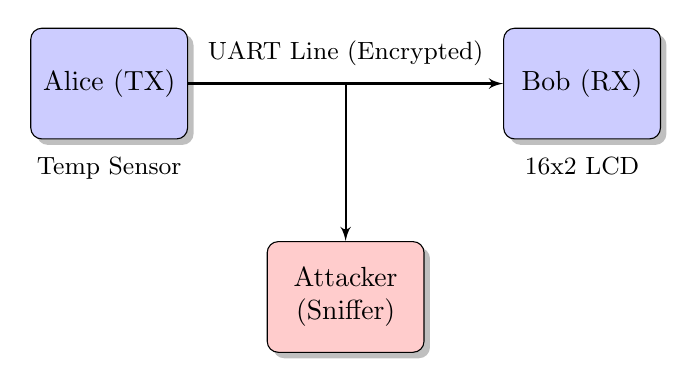
\begin{tikzpicture}[auto, node distance=4cm, >=latex']
        % Nodes
        \node [block] (alice) {Alice (TX)};
        \node [block, right=of alice] (bob) {Bob (RX)};
        \node [attacker, below=2cm of $(alice.east)!0.5!(bob.west)$] (attacker) {Attacker (Sniffer)};

        % Paths
        \draw [line] (alice) -- coordinate(mid) (bob);
        \node [above=0.1cm of mid] {\small UART Line (Encrypted)};
        \draw [line] (mid) -- (attacker);
        
        % Labels
        \node [below=0.1cm of alice] {\small Temp Sensor};
        \node [below=0.1cm of bob] {\small 16x2 LCD};
    \end{tikzpicture}
    \caption{System block diagram showing the passive sniffing architecture.}
\end{figure}

\subsection{State Machine Transitions}
To ensure synchronization during the Diffie-Hellman handshake, both nodes implement a synchronous state machine.

\begin{figure}[h]
    \centering
    \resizebox{\textwidth}{!}{
    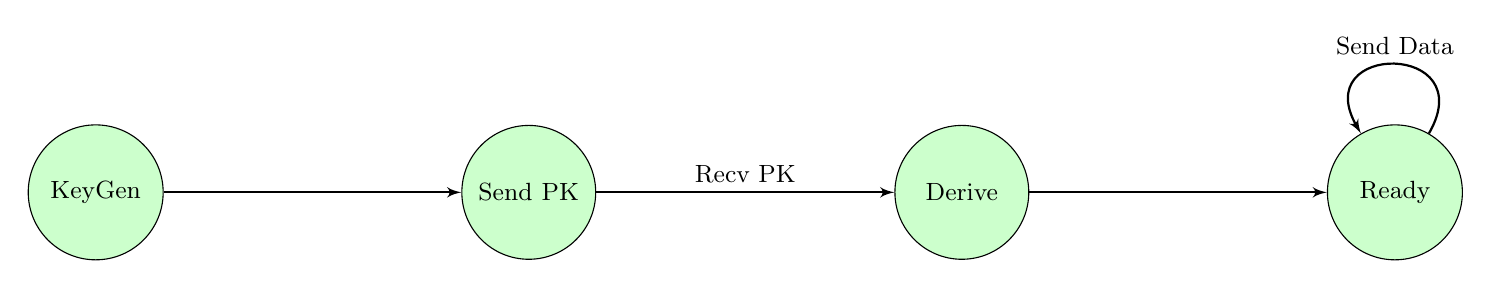
\begin{tikzpicture}[node distance=3.5cm, auto, >=latex']
        \node [state] (keygen) {\small KeyGen};
        \node [state, right of=keygen] (sendpk) {\small Send PK};
        \node [state, right of=sendpk] (derive) {\small Derive};
        \node [state, right of=derive] (ready) {\small Ready};

        \path [line] (keygen) -- (sendpk);
        \path [line] (sendpk) -- node[above] {\small Recv PK} (derive);
        \path [line] (derive) -- (ready);
        \draw [line] (ready) to [out=60, in=120, looseness=4] node[above] {\small Send Data} (ready);
    \end{tikzpicture}
    }
    \caption{Handshake and data transmission state machine.}
\end{figure}

% ---------------------------------------------------------
% 8. System Components
% ---------------------------------------------------------
\section{System Components}
\subsection{Hardware Components}
\begin{itemize}
    \item 3x Arduino Uno (ATmega328P).
    \item 2x 16x2 LCD Displays (for Bob and Attacker).
    \item LM35 Temperature Sensor.
    \item Push Button and Resistors.
\end{itemize}

\subsection{Software Stack}
\begin{itemize}
    \item Arduino IDE / C++ for firmware.
    \item DH-Lite (Custom 8-bit implementation).
    \item Speck 64/128 (Lightweight block cipher).
    \item LiquidCrystal Library for LCD interfacing.
\end{itemize}
\newpage

% ---------------------------------------------------------
% 9. Cryptographic Foundations
% ---------------------------------------------------------
\section{Cryptographic Foundations}
The security of the system relies on two distinct cryptographic primitives: one for key agreement and another for symmetric encryption.

\subsection{DH-Lite: 8-bit Diffie-Hellman}
The Diffie-Hellman (DH) protocol allows two parties to establish a shared secret over an insecure channel. In this project, we implement a lightweight version called "DH-Lite" using:
\begin{itemize}
    \item \textbf{Prime ($p$):} 251 (The largest 8-bit prime).
    \item \textbf{Generator ($g$):} 6 (A primitive root modulo 251).
\end{itemize}
The security is based on the \textit{Discrete Logarithm Problem} (DLP). While an 8-bit prime is small for modern standards, it serves as an effective proof-of-concept for resource-constrained 8-bit microcontrollers where computing $g^a \pmod p$ is instantaneous but brute-forcing the private exponent $a$ requires iterating through the entire group.

\subsection{Speck 64/128: Lightweight Block Cipher}
Speck is a family of lightweight block ciphers designed by the NSA for IoT devices. We utilize the Speck 64/128 variant:
\begin{itemize}
    \item \textbf{Block Size:} 64 bits (Split into two 32-bit words $x$ and $y$).
    \item \textbf{Key Size:} 128 bits (Four 32-bit words).
    \item \textbf{Round Function:} Uses ARX (Addition-Rotation-XOR) operations.
    \item \textbf{Number of Rounds:} 27.
\end{itemize}
Speck is chosen over AES due to its minimal RAM footprint and the absence of S-Boxes or lookup tables, which are vulnerable to side-channel timing attacks on certain hardware.

% ---------------------------------------------------------
% 10. Implementation Details
% ---------------------------------------------------------
\section{Implementation Details}
The firmware is written in C++ and optimized for the ATmega328P. Key implementation challenges included:
\begin{enumerate}
    \item \textbf{Randomness:} The initial private keys are seeded using the \textit{analogRead()} noise from an unconnected pin (A1) to ensure different shared secrets across sessions.
    \item \textbf{Framing:} A framing protocol using start (0xAA) and end (0x55) bytes ensures that Bob can synchronize with the beginning of an encrypted block even if the serial line experiences noise.
    \item \textbf{Floating Point Avoidance:} All temperature calculations for the LM35 and cryptographic operations use integer arithmetic to minimize binary size and execution time.
\end{enumerate}

% ---------------------------------------------------------
% 11. Code Snippets
% ---------------------------------------------------------
\section{Code Snippets}
\subsection{Speck Encryption Logic (Alice)}
The following snippet demonstrates the 27-round Speck encryption core using bitwise rotations and XOR operations.
\begin{lstlisting}[language=C++]
void speck_encrypt(uint32_t* x, uint32_t* y) {
  for (uint8_t i = 0; i < SPECK_ROUNDS; i++) {
    *x = (ROR32(*x, 8) + *y) ^ roundKeys[i];
    *y = ROL32(*y, 3) ^ *x;
  }
}
\end{lstlisting}

\subsection{DH-Lite Modular Exponentiation}
The modular exponentiation function is optimized for 8-bit registers by using 16-bit intermediate results to prevent overflow during multiplication.
\begin{lstlisting}[language=C++]
uint8_t dh_lite_modpow(uint8_t base, uint8_t exp, uint8_t mod) {
  uint16_t result = 1;
  uint16_t b = base % mod;
  while (exp > 0) {
    if (exp & 1) result = (result * b) % mod;
    exp >>= 1;
    b = (b * b) % mod;
  }
  return (uint8_t)result;
}
\end{lstlisting}

% ---------------------------------------------------------
% 12. Results
% ---------------------------------------------------------
\section{Results}
The system successfully established a secure link. During testing:
\begin{itemize}
    \item Alice and Bob correctly generated the same shared secret (e.g., 142).
    \item Temperature data (e.g., "TMP:25C") was correctly decrypted by Bob and displayed.
    \item The Attacker successfully intercepted the bytes but displayed them as unreadable hexadecimal values, confirming that the Speck cipher effectively obscured the payload.
\end{itemize}

% ---------------------------------------------------------
% 13. Hardware Implementation
% ---------------------------------------------------------
\section{Hardware Implementation}
% Leave empty for now as requested.

% ---------------------------------------------------------
% 14. Discussion
% ---------------------------------------------------------
\section{Discussion}
The choice of Speck 64/128 was optimal for this project because it avoids the use of heavy lookup tables (like AES), which are memory-intensive. The 8-bit DH-Lite provides a basic level of security suitable for educational purposes, though a larger prime would be required for production-level security. The dual-line sniffing proved that even with full visibility of the handshake, the discrete logarithm problem protects the shared secret.

% ---------------------------------------------------------
% 15. Conclusion
% ---------------------------------------------------------
\section{Conclusion}
This project demonstrated that end-to-end encryption is feasible on low-power microcontrollers. By combining a lightweight key exchange with a modern block cipher, we successfully secured a UART link against passive attacks. The modular design of the code allows for easy scaling to more complex sensor networks or different communication interfaces.

\end{document}
